\section{Fundamentação teórica}
\label{sec:fundamentacao}

\subsection{Conceito novo: subtração de fundo com MOG2}
\label{sec:mog2}

A subtração de fundo parte de uma ideia simples: com a câmera parada,
tudo o que difere da cena vazia é algo que entrou nela. Comparar com
uma única foto da cena vazia falha, porque nenhum pixel é constante: o
sensor tem ruído e a compressão do vídeo mexe nos valores.

O MOG (\textit{Mixture of Gaussians}) modela \textbf{cada pixel} como
uma mistura de gaussianas \citep{stauffer1999}, cada uma com uma média
$\mu$ (a cor típica), uma variância $\sigma^2$ (o quanto o pixel
costuma variar) e um peso (com que frequência aquela cor aparece).
Várias gaussianas permitem mais de um ``jeito normal'', como uma folha
que balança na frente de uma parede. O MOG2 é a versão de
\citet{zivkovic2004} e \citet{zivkovic2006}: escolhe sozinho quantas
gaussianas cada pixel precisa (até 5 no OpenCV) e detecta sombras.

Para um pixel com cor $\mathbf{x} = (B, G, R)$, o OpenCV calcula, para
as gaussianas de maior peso, a distância
\begin{equation}
D^2 = \frac{(B-\mu_B)^2 + (G-\mu_G)^2 + (R-\mu_R)^2}{\sigma^2}
\label{eq:mog2}
\end{equation}
e considera o pixel \textbf{fundo} quando $D^2 < T$, em que $T$ é o
parâmetro \texttt{varThreshold} \citep{opencv_mog2}. Dividir pela
variância é o que torna o teste justo: num pixel que varia muito, uma
diferença grande ainda é normal; numa parede lisa, uma diferença pequena
já é suspeita. O OpenCV impõe um piso de $\sigma^2 = 4$ à variância.

Se o pixel não é fundo, o MOG2 ainda testa se ele é uma
\textbf{sombra}: se a cor é a mesma do fundo, só que mais escura (entre
50\% e 100\% do brilho original), ele recebe o valor 127 em vez de 255
na saída.

Enquanto aprende, a cada quadro a gaussiana que explica a cor nova
ganha peso e tem a média puxada na direção dela, com intensidade dada
pelo \texttt{learningRate} ($-1$: o OpenCV escolhe; $0$: modelo
\textbf{congelado}). Aprendemos a cena vazia e depois congelamos, para
que uma pessoa parada não vire fundo com o tempo.

\paragraph{Exemplo feito à mão.} Considere um pixel de uma parede cinza
aprendido com $\mu = (150, 150, 150)$. Como a parede é lisa, a
variância fica no piso, $\sigma^2 = 4$. Com $T = 40$
(Tabela~\ref{tab:exemplo}):

\begin{table}[H]
\centering
\caption{Classificação de um pixel de parede ($\mu = 150$, $\sigma^2 = 4$, $T = 40$) pela Equação~\ref{eq:mog2}.}
\label{tab:exemplo}
\small
\begin{tabular}{llll}
\toprule
Cor nova $(B,G,R)$ & Conta & $D^2$ & Saída \\
\midrule
$(156, 156, 156)$ & $(6^2+6^2+6^2)/4$ & $27 < 40$ & fundo (0) \\
$(158, 158, 158)$ & $(8^2+8^2+8^2)/4$ & $48 > 40$ & frente (255) \\
$(55, 60, 45)$, camiseta & $(95^2+90^2+105^2)/4$ & $\approx 7038$ & frente (255) \\
$(120, 120, 120)$, mais escura & mesma cor, 80\% do brilho & --- & sombra (127) \\
\bottomrule
\end{tabular}
\end{table}

O exemplo mostra que, numa parede lisa, um clareamento uniforme de
apenas 8 níveis (de 0 a 255) já transforma o pixel em ``pessoa''. Em
geral, clareando $d$ níveis nos três canais, $D^2 = 3d^2/\sigma^2$, e o
pixel continua fundo enquanto $d < \sqrt{T\sigma^2/3}$, isto é,
$d < 7{,}3$ para $T = 40$ (Figura~\ref{fig:mog2}). Conferimos a conta
com uma parede sintética (cinza 150 com ruído): clareando 6 níveis,
nenhum pixel virou frente; clareando 8, 99\% viraram. Esse limite
apertado explica o maior problema que encontramos
(Seção~\ref{sec:exposicao}): quando a câmera ajusta o brilho sozinha,
a parede inteira vira ``pessoa''.

\begin{figure}[H]
\centering
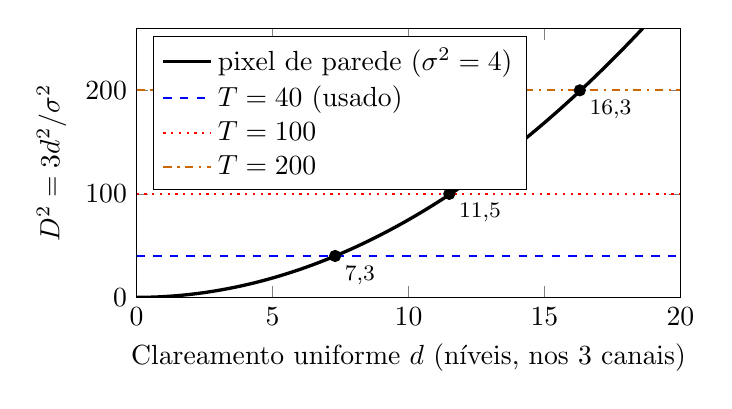
\begin{tikzpicture}
\begin{axis}[
  width=0.7\linewidth, height=5cm,
  xlabel={Clareamento uniforme $d$ (níveis, nos 3 canais)},
  ylabel={$D^2 = 3d^2/\sigma^2$},
  xmin=0, xmax=20, ymin=0, ymax=260,
  legend pos=north west, legend cell align=left]
\addplot[domain=0:20, samples=100, very thick, black] {3*x^2/4};
\addlegendentry{pixel de parede ($\sigma^2 = 4$)}
\addplot[domain=0:20, thick, dashed, blue] {40};
\addlegendentry{$T = 40$ (usado)}
\addplot[domain=0:20, thick, dotted, red] {100};
\addlegendentry{$T = 100$}
\addplot[domain=0:20, thick, dashdotted, orange!80!black] {200};
\addlegendentry{$T = 200$}
\addplot[only marks, mark=*, mark size=2pt, black] coordinates {(7.3,40) (11.5,100) (16.3,200)};
\node[anchor=north west, font=\footnotesize] at (axis cs:7.3,40) {7,3};
\node[anchor=north west, font=\footnotesize] at (axis cs:11.5,100) {11,5};
\node[anchor=north west, font=\footnotesize] at (axis cs:16.3,200) {16,3};
\end{axis}
\end{tikzpicture}
\caption{Quanto uma parede lisa pode clarear antes de virar ``pessoa'':
o pixel é fundo enquanto a curva está abaixo da linha do limiar $T$.
Figura feita pelo grupo a partir da Equação~\ref{eq:mog2}.}
\label{fig:mog2}
\end{figure}

O mesmo cálculo mostra o caso contrário, a \textbf{camuflagem}. Se a
camiseta $(55, 60, 45)$ passa na frente de um objeto escuro
$(40, 40, 40)$ cuja variância aprendida é $\sigma^2 = 25$, então
$D^2 = (15^2 + 20^2 + 5^2)/25 = 26 < 40$, e aquele pedaço da pessoa é
classificado como fundo. O MOG2 só compara cores; se a pessoa tem a cor
do que está atrás dela, ele não tem como separá-las.

\subsection{Técnicas vistas em aula}
\label{sec:tecnicas}

\textbf{Filtro gaussiano.} Substitui cada pixel por uma média ponderada
da vizinhança, com pesos maiores no centro
\citep{gonzalez2010}. Usamos um kernel $5 \times 5$ antes do MOG2 para
reduzir o ruído do sensor, que faria pixels isolados ``piscarem'' como
se fossem movimento.

\textbf{Limiarização.} Transforma uma imagem em cinza em binária: o que
está acima do limiar vira 255 e o resto vira 0 \citep{gonzalez2010}. A
saída do MOG2 tem três valores (0 fundo, 127 sombra, 255 frente);
limiarizando em 200, só a frente sobra, e a sombra que a pessoa projeta
na parede não é confundida com ela.

\textbf{Morfologia.} A erosão encolhe as regiões brancas e a dilatação
as expande, usando um elemento estruturante \citep{gonzalez2010}. A
\textbf{abertura} (erosão seguida de dilatação) apaga pontos soltos de
ruído; o \textbf{fechamento} (dilatação seguida de erosão) tapa buracos
pequenos dentro da silhueta. Usamos um elemento elíptico $7 \times 7$.

\textbf{Contornos e área.} O \texttt{findContours} encontra as bordas de
cada região branca. Descartamos as regiões com área menor que um mínimo
(manchas que a morfologia não removeu) e desenhamos as restantes
preenchidas, o que fecha buracos internos maiores. O número de regiões
que sobram é o \textbf{número de objetos}, o descritor que o programa
mostra na tela.

\textbf{Composição com borda suave.} Desfocar a máscara binária cria uma
transição de 0 a 1 na borda, o canal alfa ($\alpha$). O resultado é
$\alpha \cdot \text{quadro} + (1-\alpha) \cdot \text{fundo novo}$; sem o
desfoque, o recorte fica serrilhado.

\textbf{IoU} (\textit{Intersection over Union}). Pixels de pessoa em
comum entre duas máscaras divididos pelos pixels de pessoa em pelo
menos uma delas: 1 quando são idênticas, 0 quando não se tocam.
Preferimos o IoU à acurácia de pixels porque o fundo ocupa a maior
parte da imagem, e um programa que errasse metade da pessoa ainda teria
acurácia acima de 90\%.
